\ifdefined\COMPLETE
\else
    \input{./preambule-sacha-utf8.ltx}
    \begin{document}
\fi

\section{Fonctions dérivées}

\subsection{Exemples}

\subsubsection{Exemple \no 1}

\begin{tabular}{llll}
Soit la fonction $f :$ & $\R$ & $\longrightarrow$ & $\R$ \\
& $f$ & $\longmapsto$ & $f(x) = x^2$ \\
\end{tabular}

On a $D_f = \R$. \\

Soit $x_0 \in D_f$. \\

Montrons que $f$ est dérivable en $x_0$. \\

\begin{itemize}
\item[•] Calcul du taux d'accroissement : \vspace*{.3cm}
\\
\begin{tabular}{llll}
$T(h)$ & $=$ & $\dfrac{f(x_0 + h) - f(x_0)}{h}$ & \vspace*{.3cm} \\
& $=$ & $\dfrac{\left(x_0 + h\right)^2 - x_0^2}{h}$ & \vspace*{.3cm} \\
& $=$ & $\dfrac{x_0^2 + 2x_0h + h^2 - x_0^2}{h}$ & \vspace*{.3cm} \\
& $=$ & $\dfrac{2x_0h + h^2}{h}$ & \vspace*{.3cm} \\
& $=$ & $\dfrac{h\left(2x_0 + h\right)}{h}$ & \vspace*{.3cm} \\
& $=$ & $2x_0 + h$ & si $h \neq 0$ \\
\end{tabular} \\
\vspace*{.3cm}

\item[•] Limite du taux d'accroissement : \vspace*{.3cm}

$\lim\limits_{h \to 0} T(h) = \lim\limits_{h \to 0} (2x_0 + h) = 2x_0$ \vspace*{.3cm} \\

Donc $f$ est dérivable en $x_0$ et $f'(x_0) = 2x_0$. \\

\item[•] Fonction dérivée : \\

\begin{tabular}{llllll}
$f' :$ & $\R$ & $\longrightarrow$ & $\R$ & & \\
& $x_0$ & $\longmapsto$ & $f'(x_0)$ & $ = $ & $2x_0$ \\
& $x$ & $\longmapsto$ & $f'(x)$ & $ = $ & $2x$ \\
\end{tabular}
\end{itemize}

\vspace*{.3cm}

On a $D_{f'} = \R$

\newpage

\subsubsection{Exemple \no 2}

\begin{tabular}{llll}
Soit la fonction $f :$ & $\R$ & $\longrightarrow$ & $\R$ \\
& $f$ & $\longmapsto$ & $f(x) = x^2 - 2x - 3$ \\
\end{tabular}

On a $D_f = \R$. \\

Soit $x_0 \in D_f$. \\

Montrons que $f$ est dérivable en $x_0$. \\

\begin{itemize}
\item[•] Calcul du taux d'accroissement : \vspace*{.3cm}
\\
\begin{tabular}{llll}
$T(h)$ & $=$ & $\dfrac{f(x_0 + h) - f(x_0)}{h}$ & \vspace*{.3cm} \\
& $=$ & $\dfrac{\left[\left(x_0 + h\right)^2 -2\left(x_0 + h\right) - 3\right] - \left(x_0^2 - 2x_0 - 3\right)}{h}$ & \vspace*{.3cm} \\
& $=$ & $\dfrac{x_0^2 + 2x_0h + h^2 -2x_0 - 2h -3 -x_0^2 + 2x_0 + 3}{h}$ & \vspace*{.3cm} \\
& $=$ & $\dfrac{2x_0h + h^2 -2h}{h}$ & \vspace*{.3cm} \\
& $=$ & $\dfrac{h\left(2x_0 + h - 2\right)}{h}$ & \vspace*{.3cm} \\
& $=$ & $2x_0 + h - 2$ & si $h \neq 0$ \\
\end{tabular} \\
\vspace*{.3cm}

\item[•] Limite du taux d'accroissement : \vspace*{.3cm}

$\lim\limits_{h \to 0} T(h) = \lim\limits_{h \to 0} ( 2x_0 + h - 2) = 2x_0 - 2$ \vspace*{.3cm} \\

Donc $f$ est dérivable en $x_0$ et $f'(x_0) = 2x_0 - 2$. \\

\item[•] Fonction dérivée : \\

\begin{tabular}{llllll}
$f' :$ & $\R$ & $\longrightarrow$ & $\R$ & & \\
& $x_0$ & $\longmapsto$ & $f'(x_0)$ & $ = $ & $2x_0 - 2$ \\
& $x$ & $\longmapsto$ & $f'(x)$ & $ = $ & $2x - 2$ \\
\end{tabular}
\end{itemize}

\vspace*{.3cm}

On a $D_{f'} = \R$

\newpage

\subsubsection{Exemple \no 3}

\begin{tabular}{llll}
Soit la fonction $f :$ & $\R$ & $\longrightarrow$ & $\R$ \\
& $f$ & $\longmapsto$ & $f(x) = \dfrac{1}{x} $ \\
\end{tabular}

On a $D_f = \R \setminus \lb 0 \rb $. \\

Soit $x_0 \in D_f$. \\

Montrons que $f$ est dérivable en $x_0$. \\

\begin{itemize}
\item[•] Calcul du taux d'accroissement : \vspace*{.3cm}
\\
\begin{tabular}{llll}
$T(h)$ & $=$ & $\dfrac{f(x_0 + h) - f(x_0)}{h}$ & \vspace*{.3cm} \\
& $=$ & $\dfrac{\dfrac{1}{x_0 + h} - \dfrac{1}{x_0}}{h}$ & \vspace*{.3cm} \\
& $=$ & $\dfrac{\dfrac{x_0-\left(x_0 + h\right)}{x_0\left(x_0 + h\right)}}{h}$ & \vspace*{.3cm} \\
& $=$ & $\dfrac{\dfrac{x_0 - x_0 - h}{x_0\left(x_0 + h\right)}}{h}$ & \vspace*{.3cm} \\
& $=$ & $\dfrac{\dfrac{-h}{x_0\left(x_0 + h\right)}}{h}$ & \vspace*{.3cm} \\
& $=$ & $\dfrac{-h}{x_0\left(x_0 + h\right)} \times \dfrac{1}{h}$ & \vspace*{.3cm} \\
& $=$ & $\dfrac{-1}{x_0\left(x_0 + h\right)}$ & si $h \neq 0$ \\
\end{tabular} \\
\vspace*{.3cm}

\item[•] Limite du taux d'accroissement : \vspace*{.3cm}

$\lim\limits_{h \to 0} T(h) = \lim\limits_{h \to 0} \dfrac{-1}{x_0\left(x_0 + h\right)} = \dfrac{-1}{x_0^2}$ \vspace*{.3cm} \\

Donc $f$ est dérivable en $x_0$ et $f'(x_0) = \dfrac{-1}{x_0^2}$. \\

\item[•] Fonction dérivée : \\

\begin{tabular}{llllll}
$f' :$ & $\R$ & $\longrightarrow$ & $\R$ & & \\
& $x_0$ & $\longmapsto$ & $f'(x_0)$ & $ = $ & $\dfrac{-1}{x_0^2}$ \vspace*{.3cm} \\
& $x$ & $\longmapsto$ & $f'(x)$ & $ = $ & $\dfrac{-1}{x^2}$ \\
\end{tabular}
\end{itemize}

\vspace*{.3cm}

On a $D_{f'} = \R \setminus \lb 0 \rb $.
 
\newpage

\vspace*{-2cm}

\subsubsection{Exemple \no 4}

\begin{tabular}{llll}
Soit la fonction $f :$ & $\R$ & $\longrightarrow$ & $\R$ \\
& $f$ & $\longmapsto$ & $f(x) = \dfrac{x-1}{x+1} $ \\
\end{tabular}

On a $D_f = \R \setminus \lb -1 \rb $. \\

Soit $x_0 \in D_f$. \\

Montrons que $f$ est dérivable en $x_0$. \\

\begin{itemize}
\item[•] Calcul du taux d'accroissement : \vspace*{.3cm}
\\
\begin{tabular}{llll}
$T(h)$ & $=$ & $\dfrac{f(x_0 + h) - f(x_0)}{h}$ & \vspace*{.3cm} \\
& $=$ & $\dfrac{\dfrac{(x_0 + h) - 1}{(x_0 + h) + 1} - \dfrac{x_0 - 1}{x_0 + 1}}{h}$ & \vspace*{.3cm} \\
& $=$ & $\dfrac{\dfrac{\left(x_0 + h - 1\right)\left(x_0 + 1\right)-\left(x_0 - 1\right)\left(x_0 + h + 1\right)}{\left(x_0 + 1\right)\left(x_0 + h + 1\right)}}{h}$ & \vspace*{.3cm} \\
& $=$ & $\dfrac{\dfrac{x_0^2 + x_0 + hx_0 + h - x_0 -1 - \left(x_0^2 + hx_0 + x_0 - x_0 - h - 1\right)}{\left(x_0 + 1\right)\left(x_0 + h +1\right)}}{h}$ & \vspace*{.3cm} \\
& $=$ & $\dfrac{\dfrac{x_0^2 + x_0 + hx_0 + h - x_0 -1 - x_0^2 - hx_0 - x_0 + x_0 + h +1}{\left(x_0 + 1\right)\left(x_0 + h + 1\right)}}{h}$ & \vspace*{.3cm} \\
& $=$ & $\dfrac{\dfrac{2h}{\left(x_0 + 1\right)\left(x_0 + h + 1\right)}}{h}$ & \vspace*{.3cm} \\
& $=$ & $\dfrac{2h}{\left(x_0 + 1\right)\left(x_0 + h + 1\right)} \times \dfrac{1}{h}$ & \vspace*{.3cm} \\
& $ = $& $ \dfrac{2}{\left(x_0 + 1\right)\left(x_0 + h + 1\right)}$ & si $h \neq 0$ \\
\end{tabular} \\
\vspace*{.3cm}

\item[•] Limite du taux d'accroissement : \vspace*{.3cm}

$\lim\limits_{h \to 0} T(h) = \lim\limits_{h \to 0} \dfrac{2}{\left(x_0 + 1\right)\left(x_0 + h + 1\right)} = \dfrac{2}{\left(x_0 + 1\right)^2}$ \vspace*{.3cm} \\

Donc $f$ est dérivable en $x_0$ et $f'(x_0) = \dfrac{2}{\left(x_0 + 1\right)^2}$. \\

\item[•] Fonction dérivée : \\

\begin{tabular}{llllll}
$f' :$ & $\R$ & $\longrightarrow$ & $\R$ & & \\
& $x_0$ & $\longmapsto$ & $f'(x_0)$ & $ = $ & $\dfrac{2}{\left(x_0 + 1\right)^2}$ \vspace*{.3cm} \\
& $x$ & $\longmapsto$ & $f'(x)$ & $ = $ & $\dfrac{2}{\left(x + 1\right)^2}$ \\
\end{tabular}
\end{itemize}

\vspace*{.3cm}

On a $D_{f'} = \R \setminus \lb -1 \rb $.

\newpage

\vspace*{-1.1cm}

\subsubsection{Exemple \no 5}

\begin{tabular}{llll}
Soit la fonction $f :$ & $\R$ & $\longrightarrow$ & $\R$ \\
& $f$ & $\longmapsto$ & $f(x) = \sqrt{x} $ \\
\end{tabular}

On a $D_f = \R^+ = \left[0 \; ; \; +\infty\right[$. \\

Soit $x_0 \in D_f$. \\

Montrons que $f$ est dérivable en $x_0$. \\

\begin{itemize}
\item[•] Calcul du taux d'accroissement : \vspace*{.3cm}
\\
\begin{tabular}{llll}
$T(h)$ & $=$ & $\dfrac{f(x_0 + h) - f(x_0)}{h}$ & \vspace*{.3cm} \\
& $=$ & $\dfrac{\sqrt{x_0 + h} - \sqrt{x_0}}{h}$ & \vspace*{.3cm} \\
& $=$ & $\dfrac{\left(\sqrt{x_0 + h} - \sqrt{x_0}\right)\left(\sqrt{x_0 + h} + \sqrt{x_0}\right)}{h\sqrt{x_0 + h} + \sqrt{x_0}}$ & \vspace*{.3cm} \\
& $=$ & $\dfrac{x_0 + h - x_0}{h\left(\sqrt{x_0 + h} + \sqrt{x_0}\right)}$ & \vspace*{.3cm} \\
& $=$ & $\dfrac{h}{h\left(\sqrt{x_0 + h} + \sqrt{x_0}\right)}$ & \vspace*{.3cm} \\
& $=$ & $ \dfrac{1}{\sqrt{x_0 + h} + \sqrt{x_0}}$ & si $h \neq 0$ \vspace*{.3cm} \\
\end{tabular} \\
\vspace*{.3cm}

\item[•] Limite du taux d'accroissement : \vspace*{.3cm}

$\lim\limits_{h \to 0} T(h) = \lim\limits_{h \to 0} \dfrac{1}{h\left(\sqrt{x_0 + h} + \sqrt{x_0}\right)} = \dfrac{1}{2\sqrt{x_0}}$ \vspace*{.3cm} \\

Donc $f$ est dérivable en $x_0$ et $f'(x_0) = \dfrac{1}{2\sqrt{x_0}}$. \\

\textbf{Attention !} \\

\textbf{$\mathbf{f}$ n'est pas dérivable en $\mathbf{x_0 = 0}$} \\

\textbf{$\mathbf{f}$ est dérivable en $\mathbf{x_0 > 0}$ et $\mathbf{f'(x_0) = \dfrac{1}{2\sqrt{x_0}}}$.} \\

\item[•] Fonction dérivée : \\

\begin{tabular}{llllll}
$f' :$ & $\R$ & $\longrightarrow$ & $\R$ & & \\
& $x_0$ & $\longmapsto$ & $f'(x_0)$ & $ = $ & $\dfrac{1}{2\sqrt{x_0}}$ \vspace*{.3cm} \\
& $x$ & $\longmapsto$ & $f'(x)$ & $ = $ & $\dfrac{1}{2\sqrt{x}}$ \\
\end{tabular}
\end{itemize}

\vspace*{.3cm}

On a $D_{f'} = \R^+_* = \left]0 \; ; \; +\infty\right[$.

\newpage

\vspace*{-2cm}

\subsubsection{Exemple \no 6}

\begin{tabular}{llll}
Soit la fonction $f :$ & $\R$ & $\longrightarrow$ & $\R$ \\
& $f$ & $\longmapsto$ & $f(x) = \sqrt{x + 11} - 1 $ \\
\end{tabular}

Il faut que $x+ 11 \geqslant 0 \Longleftrightarrow x \geqslant -11$ \\

Donc on a $D_f = \left[-11 \; ; \; +\infty\right[$. \\

Soit $x_0 \in D_f$. \\

Montrons que $f$ est dérivable en $x_0$. \\

\begin{itemize}
\item[•] Calcul du taux d'accroissement : \vspace*{.3cm}
\\
\begin{tabular}{llll}
$T(h)$ & $=$ & $\dfrac{f(x_0 + h) - f(x_0)}{h}$ & \vspace*{.3cm} \\
& $=$ & $\dfrac{\sqrt{x_0 + h + 11} - 1 -\left( \sqrt{x_0 +11} - 1\right)}{h}$ & \vspace*{.3cm} \\
& $=$ & $\dfrac{\sqrt{x_0 + h + 11} - \sqrt{x_0 + 11}}{h}$ & \vspace*{.3cm} \\
& $=$ & $\dfrac{\left(\sqrt{x_0 + h + 11} - \sqrt{x_0 + 11}\right)\left(\sqrt{x_0 + h + 11} + \sqrt{x_0 + 11}\right)}{h\left(\sqrt{x_0 + h + 11} + \sqrt{x_0 + 11}\right)}$ & \vspace*{.3cm} \\
& $=$ & $\dfrac{x_0 + h + 11 - \left(x_0 + 11\right)}{h\left(\sqrt{x_0 + h + 11} + \sqrt{x_0 + 11}\right)}$ & \vspace*{.3cm} \\
& $=$ & $\dfrac{h}{h\left(\sqrt{x_0 + h + 11} + \sqrt{x_0 + 11}\right)}$ & \vspace*{.3cm} \\
& $=$ & $\dfrac{1}{{x_0 + h + 11} + \sqrt{x_0 + 11}}$ & si $h \neq 0$ \\
\end{tabular} \\
\vspace*{.3cm}

\item[•] Limite du taux d'accroissement : \vspace*{.3cm}

$\lim\limits_{h \to 0} T(h) = \lim\limits_{h \to 0} \dfrac{1}{{x_0 + h + 11} + \sqrt{x_0 + 11}} = \dfrac{1}{2\sqrt{x_0 +11}}$ \vspace*{.3cm} \\

Donc $f$ est dérivable en $x_0$ et $f'(x_0) = \dfrac{1}{2\sqrt{x_0 + 11}}$. \\

\textbf{Attention !} 

\textbf{$\mathbf{f}$ n'est pas dérivable en $\mathbf{x_0 = -11}$} 

\textbf{$\mathbf{f}$ est dérivable en $\mathbf{x_0 > -11}$ et $\mathbf{f'(x_0) = \dfrac{1}{2\sqrt{x_0 + 11}}}$.} \\

\item[•] Fonction dérivée : \\

\begin{tabular}{llllll}
$f' :$ & $\R$ & $\longrightarrow$ & $\R$ & & \\
& $x_0$ & $\longmapsto$ & $f'(x_0)$ & $ = $ & $\dfrac{1}{2\sqrt{x_0 + 11} }$ \vspace*{.3cm} \\
& $x$ & $\longmapsto$ & $f'(x)$ & $ = $ & $\dfrac{1}{2\sqrt{x + 11}}$ \\
\end{tabular}
\end{itemize}

\vspace*{.3cm}

On a $D_{f'} = \left]-11 \; ; \; +\infty\right[$.

\newpage

\subsubsection{Récapitulation}

\begin{tabular}{cccc}
Fonction primitive $f$ & Domaine de définition de $f$ & Fonction dérivée $f'$ & Domaine de définition de $f'$ \vspace*{.3cm }\\
$f(x) = x^2$ & $D_f = \R$ & $f'(x) = 2x$ & $D_{f'} = \R$ \vspace*{.3cm} \\
$f(x) = \dfrac{1}{x}$ & $D_f = \R \setminus \lb 0 \rb $ & $f'(x) = \dfrac{-1}{x^2}$ & $D_{f'} = \R \setminus \lb 0 \rb$ \vspace*{.3cm} \\
$f(x) = \sqrt{x}$ & $D_f = R^+ = \left[0 \; ; \; +\infty\right[$ & $f'(x) = \dfrac{1}{2\sqrt{x}}$ & $D_{f'} = R^+_* = \left]0 \; ; \; +\infty\right[$ \vspace*{.3cm} \\
\end{tabular}

\newpage

\subsection{Dérivée de la fonction constante et dérivée de la fonction identité}

\subsubsection{Dérivée de la fonction constante}

\begin{tabular}{llll}
Soit la fonction $f :$ & $\R$ & $\longrightarrow$ & $\R$ \\
& $f$ & $\longmapsto$ & $f(x) = a$ \\
\end{tabular}

On a $D_f = \R$. \\

Soit $x_0 \in D_f$. \\

Montrons que $f$ est dérivable en $x_0$. \\

\begin{itemize}
\item[•] Calcul du taux d'accroissement : \vspace*{.3cm}
\\
\begin{tabular}{llll}
$T(h)$ & $=$ & $\dfrac{f(x_0 + h) - f(x_0)}{h}$ & \vspace*{.3cm} \\
& $=$ & $\dfrac{a - a}{h}$ & \vspace*{.3cm} \\
& $=$ & $0$ & si $h \neq 0$ \\
\end{tabular} \\
\vspace*{.3cm}

\item[•] Limite du taux d'accroissement : \vspace*{.3cm}

$\lim\limits_{h \to 0} T(h) = 0$ \\

Donc $f$ est dérivable en $x_0$ et $f'(x_0) = 0$. \\

\item[•] Fonction dérivée : \\

\begin{tabular}{llllll}
$f' :$ & $\R$ & $\longrightarrow$ & $\R$ & & \\
& $x_0$ & $\longmapsto$ & $f'(x_0)$ & $ = $ & $0$ \\
& $x$ & $\longmapsto$ & $f'(x)$ & $ = $ & $0$ \vspace*{.3cm} \\
\end{tabular}
\end{itemize}

\vspace*{.3cm}

On a $D_{f'} = \R$. \\

On peut retenir que \textbf{la dérivée d'une constante est nulle.}

\newpage

\subsubsection{Dérivée de la fonction identité}

\begin{tabular}{llll}
Soit la fonction $f :$ & $\R$ & $\longrightarrow$ & $\R$ \\
& $f$ & $\longmapsto$ & $f(x) = x$ \\
\end{tabular}

On a $D_f = \R$. \\

Soit $x_0 \in D_f$. \\

Montrons que $f$ est dérivable en $x_0$. \\

\begin{itemize}
\item[•] Calcul du taux d'accroissement : \vspace*{.3cm}
\\
\begin{tabular}{llll}
$T(h)$ & $=$ & $\dfrac{f(x_0 + h) - f(x_0)}{h}$ & \vspace*{.3cm} \\
& $=$ & $\dfrac{x_0 + h - x_0}{h}$ & \vspace*{.3cm} \\
& $=$ & $\dfrac{h}{h}$ & \vspace*{.3cm} \\
& $=$ & $1$ & si $h \neq 0$ \\
\end{tabular} \\
\vspace*{.3cm}

\item[•] Limite du taux d'accroissement : \vspace*{.3cm}

$\lim\limits_{h \to 0} T(h) = 1$ \\

Donc $f$ est dérivable en $x_0$ et $f'(x_0) = 1$. \\

\item[•] Fonction dérivée : \\

\begin{tabular}{llllll}
$f' :$ & $\R$ & $\longrightarrow$ & $\R$ & & \\
& $x_0$ & $\longmapsto$ & $f'(x_0)$ & $ = $ & $1$ \\
& $x$ & $\longmapsto$ & $f'(x)$ & $ = $ & $1$ \vspace*{.3cm} \\
\end{tabular}
\end{itemize}

\vspace*{.3cm}

On a $D_{f'} = \R$. \\

On peut retenir que \textbf{la dérivée de $\mathbf{x}$ est $\mathbf{1}$.}

\newpage

\subsection{Formules fondamentales}

Soient $u$ et $v$ deux fonctions dérivables. \\ Soient $u'$ et $v'$ leur fonction dérivée respectives. 

\subsubsection{Dérivée de la somme de deux fonctions}

$\mathbf{\left(u + v\right)^{'} = u' + v'}$ \\

\textbf{Exemple :} \\

\begin{tabular}{llll}
Soit la fonction $f :$ & $\R$ & $\longrightarrow$ & $\R$ \\
& $x$ & $\longmapsto$ & $f(x) = x + 8$ \\
\end{tabular}

\vspace*{.3cm}

On a : \\

\begin{itemize}
\item[•] $u\left(x\right) = x$
\item[•] $v\left(x\right) = 8$
\item[•] $u'\left(x\right) = 1$
\item[•] $v'\left(x\right) = 0$
\end{itemize}

Donc $f'(x) = 1 + 0 = 1$ 

\subsubsection{Dérivée du produit d'une fonction par un nombre réel}

$\mathbf{\left(\lambda u\right)^{'} = \lambda u'}$ \\

\textbf{Exemple :} \\

\begin{tabular}{llll}
Soit la fonction $f :$ & $\R$ & $\longrightarrow$ & $\R$ \\
& $x$ & $\longmapsto$ & $f(x) = 5x$ \\
\end{tabular}

\vspace*{.3cm}

On a : \\

\begin{itemize}
\item[•] $u\left(x\right) = x$
\item[•] $u'\left(x\right) = 1$
\item[•] $\lambda = 5$
\end{itemize}

Donc $f'(x) = 5 \times x = 5x$ \\

\newpage

\subsubsection{Dérivée du produit de deux fonctions}

$\mathbf{\left(uv\right)^{'} = u'v + uv'}$ \\

\textbf{Exemples :} \\

\textbf{Exemple n°1 :} \\

\begin{tabular}{llll}
Soit la fonction $f :$ & $\R$ & $\longrightarrow$ & $\R$ \\
& $x$ & $\longmapsto$ & $f(x) = x^2$ \\
\end{tabular}

\vspace*{.3cm}

$f(x) = x \times x$ \\

On a : \\

\begin{itemize}
\item[•] $u\left(x\right) = x$
\item[•] $v\left(x\right) = x$
\item[•] $u'\left(x\right) = 1$
\item[•] $v'\left(x\right) = 1$
\end{itemize}

\vspace*{.3cm}

\begin{tabular}{lll}
Donc $f(x)$ & $=$ & $1 \times x + x \times 1$ \\
& $=$ & $x + x$ \\
& $=$ & $2x$ \\
\end{tabular}

\vspace*{.3cm}

Donc $f'(x) = 2x$. \\

\textbf{Exemple n°2 :} \\

\begin{tabular}{llll}
Soit la fonction $f :$ & $\R$ & $\longrightarrow$ & $\R$ \\
& $x$ & $\longmapsto$ & $f(x) = x^3$ \\
\end{tabular}

\vspace*{.3cm}

$f(x) = x^2 \times x$ \\

On a : \\

\begin{itemize}
\item[•] $u\left(x\right) = x^2$
\item[•] $v\left(x\right) = x$
\item[•] $u'\left(x\right) = 2x$
\item[•] $v'\left(x\right) = 1$
\end{itemize}

\vspace*{.3cm}

\begin{tabular}{lll}
Donc $f(x)$ & $=$ & $2x \times x + x^2 \times 1$ \\
& $=$ & $2x^2 + x^2$ \\
& $=$ & $3x^2$ \\
\end{tabular}

Donc $f'(x) = 3x^2$. 

\newpage

\textbf{Exemple n°3 :} \\

\begin{tabular}{llll}
Soit la fonction $f :$ & $\R$ & $\longrightarrow$ & $\R$ \\
& $x$ & $\longmapsto$ & $f(x) = x^4$ \\
\end{tabular}

\vspace*{.3cm}

$f(x) = x^3 \times x$ \\

On a : \\

\begin{itemize}
\item[•] $u\left(x\right) = x^3$
\item[•] $v\left(x\right) = x$
\item[•] $u'\left(x\right) = 3x^2$
\item[•] $v'\left(x\right) = 1$
\end{itemize}

\vspace*{.3cm}

\begin{tabular}{lll}
Donc $f(x)$ & $=$ & $3x^2 \times x + x^3 \times 1$ \\
& $=$ & $3x^3 + x^3$ \\
& $=$ & $4x^3$ \\
\end{tabular}

\vspace*{.3cm}

Donc $f'(x) = 4x^3$. \\

\textbf{On conjecture que :} \\

\begin{tabular}{llll}
\textbf{Soit la fonction }$\mathbf{f} :$ & $\mathbf{\R}$ & $\mathbf{\longrightarrow}$ & $\mathbf{\R}$ \\
& $\mathbf{x}$ & $\mathbf{\longmapsto}$ & $\mathbf{f(x)}$ \\
\end{tabular}

\vspace*{.3cm}

$\mathbf{\forall n \geqslant 1, f(x) = nx^{n-1}}$ \\

\textbf{Exercices d'application : dérivées de fonctions polynômes} \\

\textbf{Exercice n°1} \\

\begin{tabular}{llll}
Soit la fonction $f :$ & $\R$ & $\longrightarrow$ & $\R$ \\
& $x$ & $\longmapsto$ & $f(x) = x^2 - 2x - 3$ \\
\end{tabular}

\vspace*{.3cm}

On a donc $f'(x) = 2x - 2$ \\

\textbf{Exercice n°2} \\

\begin{tabular}{llll}
Soit la fonction $f :$ & $\R$ & $\longrightarrow$ & $\R$ \\
& $x$ & $\longmapsto$ & $f(x) = 30x^4 - 23x^3 + 11x^2 -48x +100$ \\
\end{tabular}

\vspace*{.3cm}

\begin{tabular}{lll}
$f'(x)$ & $=$ & $ 120x^3 - 69x^2 + 22x - 48 $ \\
$f''(x)$ & $=$ & $ 360x^2 - 138x + 22 $ \\
$f'''(x)$ & $=$ & $ 720 x - 138$ \\
$f''''(x)$ & $=$ & $ 720$ \\
\end{tabular}

\newpage

\subsubsection{Dérivée des puissances d'une fonction}

\begin{itemize}
\item[•] $\mathbf{\left(u^2\right)^{'} = 2uu'}$ \\

En effet, $u^2 = u \times u$. \\

\begin{tabular}{lll}
D'où $\left(u^2\right)^{'}$ & $ = $ & $ u'u + uu' $ \\
& $=$ & $uu' + uu'$ \\
& $=$ & $2uu'$ \\
\end{tabular}

\vspace*{.3cm}

\item[•] $\mathbf{\left(u^3\right)^{'} = 3u^2u'}$ \\

En effet, $u^3 = u^2 \times u$. \\

\begin{tabular}{lll}
D'où $\left(u^3\right)^{'}$ & $ = $ & $ \left(2uu'\right)u + u^2u' $ \\
& $=$ & $2u^2u' + u^2u'$ \\
& $=$ & $3u^2u'$ \\
\end{tabular}

\vspace*{.3cm}

\item[•] $\mathbf{\left(u^4\right)^{'} = 4u^3u'}$ \\

En effet, $u^4 = u^3 \times u$. \\

\begin{tabular}{lll}
D'où $\left(u^4\right)^{'}$ & $ = $ & $ \left(3u^2u'\right)u + u^3u' $ \\
& $=$ & $3u^3u' + u^3u'$ \\
& $=$ & $4u^3u'$ \\
\end{tabular}

\vspace*{.3cm}

\item[•] \textbf{On conjecture que :} \\

$\mathbf{\left(u^n\right)^{'} = nu^{n-1}u'}$
\end{itemize}

\vspace*{.3cm}

\textbf{Exercices} \\

\textbf{Exercice n°1} \\

\begin{tabular}{llll}
Soit la fonction $f :$ & $\R$ & $\longrightarrow$ & $\R$ \\
& $x$ & $\longmapsto$ & $f(x) = \left(5x + 7\right)^2$ \\
\end{tabular}

\vspace*{.3cm}

Calculer $f'(x)$ de deux manières. \\

\begin{itemize}
\item[•] Première méthode : \\

\begin{tabular}{llll}
& $f(x)$ & $ = $ & $25x^2 + 70x + 39$ \vspace*{.3cm} \\
D'où & $f'(x) $ & $=$ & $ 50x + 70$ \\
\end{tabular}

\vspace*{.3cm}

\item[•] Seconde méthode : \\

$u(x) = 5x + 7$ et $u'(x) = 5$ \\

\begin{tabular}{lll}
D'où $f'(x)$ & $=$ & $2\left(5x + 7\right) \times 5$ \\
& $=$ & $10\left(5x + 7\right) $ \\
& $=$ & $50x + 70$ \\
\end{tabular}
\end{itemize}

\newpage

\textbf{Exercice n°3 : Plus musclé} \\

\begin{tabular}{llll}
Soit la fonction $f :$ & $\R$ & $\longrightarrow$ & $\R$ \\
& $x$ & $\longmapsto$ & $f(x) = \left(x^2 - 2x - 3\right)^2 \left(2x - 6\right)^3$ \\
\end{tabular}

\vspace*{.3cm}

\begin{itemize}
\item[•] $u(x) = \left(x^2 - 2x - 3\right)^2$ \\
\item[•] $v(x) = \left(2x -6\right)^3$ \\
\item[•] $u'(x) = 2\left(x^2 -2x - 3\right)\left(2x - 2\right)$ \\
\item[•] $v'(x) = 3\left(2x - 6\right)^2 \times 2$ \\
\end{itemize}

\begin{tabular}{lll}
D'où $f'(x)$ & $ = $ & $ 2\left(x^2 -2x - 3\right)\left(2x - 2\right)\left(2x -6\right)^3 + \left(x^2 - 2x - 3\right)^2 \times 3\left(2x - 6\right)^2 \times 2$ \vspace*{.3cm} \\
& $=$ & $2\left(x^2 - 2x - 3\right)\left(2x - 6\right)^2\left[\left(2x - 2\right)\left(2x - 6\right) + \left(x^2 - 2x - 3\right) \times 3\right]$ \vspace*{.3cm} \\
& $=$ & $2\left(x^2 - 2x - 3\right)\left(2x - 6\right)^2\left(4x^2 - 16x + 12 + 3x^2 - 6x - 9\right)$ \vspace*{.3cm} \\
& $=$ & $2\left(x^2 - 2x - 3\right)\left(2x - 6\right)^2\left(7x^2 - 22x +3\right)$ \\
\end{tabular}

\vspace*{.3cm}

Encore plus fort ? On peut continuer de factoriser ! \\

On a : \\

\begin{itemize}
\item[•] $x^2 - 2x - 3 = \left(x-3\right)\left(x+1\right)$ \\
\item[•] $2x - 6 = 2\left(x -3\right)$ \\
\item[•] $7x^2 - 22x + 3 = \left(x-3\right)\left(x-\dfrac{1}{7}\right)$ \\
\end{itemize}

\vspace*{.3cm}

\begin{tabular}{lll}
Donc $f'(x)$ & $=$ & $2\left(x^2 - 2x - 3\right)\left(2x - 6\right)^2\left(7x^2 - 22x +3\right)$ \\
& $=$ & $2\left(x-3\right)\left(x+1\right)\left[2\left(x-3\right)\right]^2\left(x-3\right)\left(x-\dfrac{1}{7}\right)$ \\ 
& $=$ & $2\left(x-3\right)\left(x+1\right) \times 4\left(x-3\right)^2 \times \left(x-3\right)\left(x-\dfrac{1}{7}\right)$ \\
& $=$ & $8\left(x-3\right)^4\left(x+1\right)\left(x-\dfrac{1}{7}\right)$ \\
\end{tabular}

\vspace*{.3cm}

Donc $f'(x) = 8\left(x-3\right)^4\left(x+1\right)\left(x-\dfrac{1}{7}\right)$ 

\newpage

\subsubsection{Dérivée de l'inverse d'une fonction}

$\mathbf{\left(\dfrac{1}{u}\right)^{'} = \dfrac{-u^{'}}{u^2}}$ \\

\textbf{Exercice n°0} \\

\begin{tabular}{llll}
Soit la fonction $f :$ & $\R$ & $\longrightarrow$ & $\R$ \\
& $x$ & $\longmapsto$ & $f(x) =  \dfrac{1}{x}$ \\
\end{tabular}

\vspace*{.3cm}

On a $D_f = \R \setminus \lb 0 \rb $ \\

$f'(x) = \dfrac{-1}{x^2}$ \\

\textbf{Exercice n°1} \\

\begin{tabular}{llll}
Soit la fonction $f :$ & $\R$ & $\longrightarrow$ & $\R$ \\
& $x$ & $\longmapsto$ & $f(x) = \dfrac{1}{x^2 - 2x - 3} $ \\
\end{tabular}

\vspace*{.3cm}

On a $D_f = \left]-\infty \; ; \; -1\right[\cup\left]-1\; ; \; 3\right[\cup \left]3 \; ; \; +\infty\right[$. \\

$f'(x) = \dfrac{-\left(2x - 2\right)}{\left(x^2 - 2x - 3\right)^2}$ \vspace*{.3cm} \\

Donc $f'(x) = \dfrac{-2x + 2}{\left(x^2 - 2x - 3\right)^2}$ \vspace*{.3cm} \\

\textbf{Exercice n°2} \\

\begin{tabular}{llll}
Soit la fonction $f :$ & $\R$ & $\longrightarrow$ & $\R$ \\
& $x$ & $\longmapsto$ & $f(x) = \dfrac{1}{\left(2x - 6\right)^3} $ \\
\end{tabular}

\vspace*{.3cm}

Il ne faut pas que $\left(2x - 6\right)^3 = 0 \Longleftrightarrow x = 3$. \\

On a :

\begin{itemize}
\item[•] $u(x) = \left(2x - 6\right)^3$ \\
\item[•] $u'(x) = 3\left(2x - 6\right)^2 \times 2 = 6\left(2x - 6\right)^2$ \\
\end{itemize}

\vspace*{.3cm}

Alors $f'(x) = \dfrac{-6\left(2x - 6\right)^2}{\left(2x - 6\right)^6}$ \\

Donc $f'(x) = \dfrac{-6}{\left(2x - 6\right)^4}$ \\

\newpage

\subsubsection{Dérivée du quotient de deux fonctions}

$\mathbf{\left(\dfrac{u}{v}\right)^{'} = \dfrac{u'v - uv'}{v^2}}$ \\

\textbf{Exercice n°0} \\

\begin{tabular}{llll}
Soit la fonction $f :$ & $\R$ & $\longrightarrow$ & $\R$ \\
& $x$ & $\longmapsto$ & $f(x) = \dfrac{x - 1}{x + 1} $ \\
\end{tabular}

\vspace*{.3cm}

$D_f = \R \setminus \lb -1 \rb $ \\

$f'(x) = \dfrac{1\left(x+1\right) - \left(x-1\right)\times 1}{\left(x+1\right)^2}$ \vspace*{.3cm} \\

Donc $f'(x) = \dfrac{2}{\left(x+1\right)^2}$ \vspace*{.3cm} \\

\textbf{Exercice n°1} \\

\begin{tabular}{llll}
Soit la fonction $f :$ & $\R$ & $\longrightarrow$ & $\R$ \\
& $x$ & $\longmapsto$ & $f(x) = \dfrac{x^2 + 4 }{x^2 - 4} $ \\
\end{tabular}

$D_f = \left]-\infty \; ; \; -2\right[\cup \left]-2 \; ; \; 2\right[\cup \left]2 \; ; \; +\infty\right[$. \\

\begin{tabular}{lll}
$ f'(x)$ & $=$ & $\dfrac{2x\left(x^2 - 4\right)- \left(x^2 + x\right) \times 2x}{\left(x^2 -4\right)^2}$ \vspace*{.3cm} \\
& $=$ & $\dfrac{2x^3 - 8x - 2x^3 -8x}{\left(x^2 -4\right)^4}$ \vspace*{.3cm} \\
& $=$ & $\dfrac{-16x}{\left(x^2 - 4\right)^2}$ \\
\end{tabular}

\vspace*{.3cm}

Donc $f'(x) = \dfrac{-16x}{\left(x^2 - 4\right)^2}$ \vspace*{.3cm} \\

\newpage

\textbf{Exercice n°2} \\

\begin{tabular}{llll}
Soit la fonction $f :$ & $\R$ & $\longrightarrow$ & $\R$ \\
& $x$ & $\longmapsto$ & $f(x) = \dfrac{2x^2 + x - 13}{x^2 - x - 2} $ \\
\end{tabular}

\vspace*{.3cm}

Il ne faut que que $x^2 - x - 2 = 0$. Donc il ne faut pas que $x = -1$ ou $x=2$ \\ 

On a $D_f = \left]-\infty \; ; \; -1\right[ \cup \left]-1 \; ; \; 2 \right[\cup \left]2 \; ; \; +\infty\right[$. \\

On a

\begin{itemize}
\item[•] $u(x) = 2x^2 + x - 13$
\item[•] $v(x) = x^2 - x - 2$
\item[•] $u'(x) = 4x + 1$
\item[•] $v'(x) = 2x - 1$ 
\end{itemize}


\vspace*{.3cm}

\begin{tabular}{lll}
Ainsi, $f'(x)$ & $=$ & $\dfrac{\left(4x +1\right)\left(x^2 _ x - 2\right)-\left(2x - 1\right)\left(2x^2 + x - 13\right)}{\left(x^2 - x - 2\right)^2}$ \vspace*{.3cm} \\
& $=$ & $\dfrac{4x^3 _ 4x^2 - 8x + x^2 -x - 2-\left(4x^3 + 2x^2 - 26x - 2x^2 -x + 13\right)}{\left(x^2 - x - 2\right)^2}$ \vspace*{.3cm} \\
& $=$ & $\dfrac{4x^3 - 3x^2 - 9x - 2 - 4x^2 - 2x^2 + 26x + 2x^2 + x - 13}{\left(x^2 - x -2\right)^2}$ \vspace*{.3cm} \\
& $=$ & $\dfrac{-3x^2 + 18x - 15}{\left(x^2 - x - 2\right)^2}$ \vspace*{.3cm} \\ 
\end{tabular}

Donc $f'(x) = \dfrac{-3x^2 + 18x - 15}{\left(x^2 - x - 2\right)^2}$. 

\newpage

\vspace*{-2cm}

\textbf{Exercice pour élèves musclés :}

\begin{tabular}{llll}
Soit la fonction $f :$ & $\R$ & $\longrightarrow$ & $\R$ \\
& $x$ & $\longmapsto$ & $f(x) =  \dfrac{\left(3x+2\right)^2}{\left(5x^2 + 6x + 1\right)^3} $ \\
\end{tabular}

Il ne faut pas que $\left(5x^2 + 6x + 1\right)^3 = 0$. Il ne faut donc pas que $x = -1$ ou $x = -\dfrac{1}{5}$. \\

D'où $D_f = \R \setminus \lb -\dfrac{1}{5} \; ; \; -1 \rb$. \\

\begin{itemize}
\item[•] $u(x) = \left(3x + 2\right)^2$
\item[•] $v(x) = \left(5x^2 + 6x + 1\right)^3$
\item[•] $u'(x) = 2\left(3x + 2\right)\times 3$
\item[•] $v'(x) = 3\left(3x^2 + 6x + 1\right)^2 \times \left(10+6\right)$
\end{itemize}

\vspace*{.3cm}

\begin{tabular}{lll}
$f'(x)$ & $=$ & $\dfrac{2\left(3x + 2\right) \times 3\left(5x^2 + 6x + 1\right)^3 - 3\left(3x^2 + 6x + 1\right)^2 \times \left(10+6\right)\left(3x + 2\right)^2}{\left(5x^2 + 6x + 1\right)^6}$ \vspace*{.3cm} \\ 
& $=$ & $\dfrac{3\left(3x + 2\right)\left(5x^2 + 6x + 1\right)^2\left[2\left(5x^2 + 6x + 1\right) - \left(10x + 6\right)\left(3x +2 \right)\right]}{\left(5x^2 + 6x + 1\right)^6}$ \vspace*{.3cm} \\ 
& $=$ & $\dfrac{3\left(3x + 2\right)\left[10x^2 + 12x + 2 - \left(30x^2 + 20x + 18x + 12\right)\right]}{\left(5x^2 + 6x + 1\right)^4}$ \vspace*{.3cm} \\ 
& $=$ & $\dfrac{3\left(3x + 2\right)\left(10x + 12x + 2 - 30x^2 - 38x - 12\right)}{\left(5x^2 + 6x + 1\right)^4}$ \vspace*{.3cm} \\ 
& $=$ & $\dfrac{3\left(3x + 2\right)\left(-20x^2 - 26x - 10\right)}{\left(5x^2 + 6x + 1\right)^4}$ \vspace*{.3cm} \\ 
& $=$ & $\dfrac{-6\left(3x + 2\right)\left(10x^2 + 13x + 5\right)}{\left(5x^2 + 6x + 1\right)^4}$ \vspace*{.3cm} \\ 
\end{tabular}

Donc $f'(x) = \dfrac{-6\left(3x + 2\right)\left(10x^2 + 13x + 5\right)}{\left(5x^2 + 6x + 1\right)^4}$.

\subsubsection{Supplément gratuit : Dérivée de la racine carrée d'une fonction}

$\mathbf{\left(\sqrt{u}\right)' = \dfrac{u'}{2\sqrt{u}}}$ \\

\textbf{Exercice n°1} \\

\begin{tabular}{llll}
Soit la fonction $f :$ & $\R$ & $\longrightarrow$ & $\R$ \\
& $x$ & $\longmapsto$ & $f(x) =  \sqrt{x} $ \\
\end{tabular}

\vspace*{.3cm}

Il faut que $x \geqslant 0$. Donc $D_f = \left[0 \; ; \; +\infty \right[$. \\

$f'(x) = \dfrac{1}{2\sqrt{x}}$ \\

\textbf{Exercice n°2} \\

\begin{tabular}{llll}
Soit la fonction $f :$ & $\R$ & $\longrightarrow$ & $\R$ \\
& $x$ & $\longmapsto$ & $f(x) =  \sqrt{x+11} - 1 $ \\
\end{tabular}

\vspace*{.3cm}

Il faut que $x +11 \geqslant 0 \Longleftrightarrow x \geqslant -11$. Donc $D_f = \left[-11 \; ; \; +\infty \right[$. \\

$f'(x) = \dfrac{1}{2\sqrt{x + 11}}$, avec $D_{f'} = \left]-11 \; ; \; +\infty \right[$

\vspace*{-5cm}

\newpage

%
%
%
%
%
%
%
%
%
%
%
%
%
%
%
%
%
\subsection{Dérivées successives}

\subsubsection{Exemples}

\textbf{Exemple n°1} \\

\begin{tabular}{llll}
Soit la fonction $f :$ & $\R$ & $\longrightarrow$ & $\R$ \\
& $x$ & $\longmapsto$ & $f(x) = x^4$ \\
\end{tabular}

\vspace*{.3cm}

On a $D_f = \R$. \\

$f' \left(x\right) = 4x^3$ \\
$f'' \left(x\right) = 12 x^2$ \\
$f'''\left(x\right) = 24x$ \\
$f^{(4)} = 24$ \\
$f^{(5)} = 0$ \\
... \\
$f^{(n)} = 0$ si $n \geqslant 5$ \\

\textbf{Exemple n°2} \\

\begin{tabular}{llll}
Soit la fonction $f :$ & $\R$ & $\longrightarrow$ & $\R$ \\
& $x$ & $\longmapsto$ & $f(x) = \dfrac{1}{x}$ \\
\end{tabular}

\vspace*{.3cm}

On a $D_f = \R \setminus \lb 0 \rb$. \\

$f' \left(x\right) = \dfrac{-1}{x^2}$ \vspace*{.3cm} \\

$f''\left(x\right) = \left(-1 \times \dfrac{1}{x^2}\right)^{'} = -1 \times \dfrac{-2x}{x^4} = \dfrac{2}{x^3}$ \vspace*{.3cm} \\

$f''' \left(x\right) = \left(2 \times \dfrac{1}{x^3}\right)^{'} = 2 \times \dfrac{-3x^2}{x^6} = \dfrac{-6}{x^4}$ \vspace*{.3cm} \\

$f^{(4)} \left(x\right) = \left( -6 \times \dfrac{1}{x^4}\right)^{'} = -6 \times \dfrac{-4x^3}{x^8} = \dfrac{24}{x^5}$ \vspace*{.3cm} \\ 

... \vspace*{.3cm} \\
 
$f^{(n)} \left(x\right) = \dfrac{\left(-1\right)^n n!}{x^{n+1}}$. \\

\newpage

\vspace*{-1.4cm}

\textbf{Exemple n°3} \\

\begin{tabular}{llll}
Soit la fonction $f :$ & $\R$ & $\longrightarrow$ & $\R$ \\
& $x$ & $\longmapsto$ & $f(x) = \dfrac{x-1}{x+1}$ \\
\end{tabular}

On a $D_f = \R \setminus \lb -1 \rb$. \\

$f' \left(x\right) = \dfrac{2}{\left(x+1\right)^2}$ \vspace*{.3cm} \\

$f''\left(x\right) = \left(2 \times \dfrac{1}{\left(x+1\right)^2}\right)^{'} = 2 \times \dfrac{-2\left(x+1\right) \times 1}{\left(x+1\right)^4} =  \dfrac{-4\left(x+1\right)}{\left(x+1\right)^4} = \dfrac{-4}{\left(x+1\right)^3}$ \vspace*{.3cm} \\

$f'''\left(x\right) = \left(-4 \times \dfrac{1}{\left(x+1\right)^3}\right)^{'} = -4 \times \dfrac{-3\left(x+1\right)^2 \times 1}{\left(x+1\right)^6} =  \dfrac{12\left(x+1\right)^2}{\left(x+1\right)^6} = \dfrac{12}{\left(x+1\right)^4}$ \vspace*{.3cm} \\

$f^{(4)}\left(x\right) = \left(12 \times \dfrac{1}{\left(x+1\right)^4}\right)^{'} = 12 \times \dfrac{-4\left(x+1\right)^3 \times 1}{\left(x+1\right)^{8}} =  \dfrac{-48\left(x+1\right)^3}{\left(x+1\right)^8} = \dfrac{-48}{\left(x+1\right)^5}$ \vspace*{.3cm} 

... \vspace*{.3cm} 

$f^{(n)} = \dfrac{2n!\left(-1\right)^{n+1}}{\left(x+1\right)^{n+1}}$ \\

\textbf{Exemple n°4} \\

\begin{tabular}{llll}
Soit la fonction $f :$ & $\R$ & $\longrightarrow$ & $\R$ \\
& $x$ & $\longmapsto$ & $f(x) = \dfrac{5x-1}{2x-3}$ \\
\end{tabular}

On a $D_f = \R \setminus \lb \dfrac{3}{2} \rb$. \vspace*{.3cm} \\

$f'(x) = \dfrac{5\left(2x - 3\right)-2\left(5x-1\right)}{\left(2x-3\right)^2}$ \vspace*{.3cm} \\

$f'(x) = \dfrac{10x - 15 - 10x + 2}{\left(2x - 3\right)^2}$ \vspace*{.3cm} \\

$f'(x) = \dfrac{-13}{\left(2x - 3\right)^2}$ \vspace*{.3cm} \\

De même, on a : $f''(x) = \left(-13 \times \dfrac{1}{\left(2x - 3\right)^2}\right)^{'} = -13 \times \dfrac{-2\left(2x - 3\right)}{\left(2x - 3\right)^4} = \dfrac{26}{\left(2x - 3\right)^3}$ \vspace*{.3cm} \\

$f^{(3)}(x) = \left(26 \times \dfrac{1}{\left(2x - 3\right)^3}\right)^{'} = 26 \times \dfrac{-3\left(2x - 3\right)^2}{\left(2x - 3\right)^6} = \dfrac{-78}{\left(2x - 3\right)^4}$ \vspace*{.3cm} \\

$f^{(4)}(x) = \left(-78 \times \dfrac{1}{\left(2x - 3\right)^4}\right)^{'} = -78 \times \dfrac{-4\left(2x - 3\right)^3}{\left(2x - 3\right)^8} = \dfrac{312}{\left(2x - 3\right)^5}$ \vspace*{.3cm} \\

$f^{(5)}(x) = \left(312 \times \dfrac{1}{\left(2x - 3\right)^5}\right)^{'} = 312 \times \dfrac{-5\left(2x - 3\right)^4}{\left(2x - 3\right)^{10}} = \dfrac{-1560}{\left(2x - 3\right)^6}$ \vspace*{.3cm} 

... \vspace*{.3cm} 

$f^{(n)} = \dfrac{13n!\left(-1\right)^{n}}{\left(2x-3\right)^{n+1}}$

\newpage

\subsection{Tableau récapitulatif}

Soient $u$ et $v$ deux fonctions définies sur un intervalle I. On a : \\

\begin{tabular}{rlll}
$\left(u + v\right)'$ & $=$ & $u' + v' $ & \vspace*{.3cm} \\
$\left(\lambda u\right)'$ & $=$ & $\lambda u'$ & \vspace*{.3cm} \\
$\left(uv\right)'$ & $=$ & $u'v + uv'$ & \vspace*{.3cm} \\
$\left(u^n\right)'$ & $ = $ & $ nu^{n-1}u'$ & \vspace*{.3cm} \\
$\left(\dfrac{1}{u}\right)'$ & $=$ & $\dfrac{-u'}{u^2}$ & \vspace*{.3cm} \\
$\left(\dfrac{u}{v}\right)'$ & $=$ & $\dfrac{u'v - uv'}{v^2}$ & Si $v$ ne s'annule pas sur $I$. \vspace*{.3cm} \\
$\left(\sqrt{u}\right)'$ & $=$ & $\dfrac{u'}{2\sqrt{u}}$ & \vspace*{.3cm} \\
\end{tabular}

\newpage

\subsection{Exercices}

\subsubsection{Exercice \no 1}

\begin{tabular}{llll}
Soit la fonction $f :$ & $\R$ & $\longrightarrow$ & $\R$ \\
& $x$ & $\longmapsto$ & $f(x) = \left(4x - 5\right)^3$ \\
\end{tabular}

\vspace*{.3cm}

On a $D_f = \R$. \\

Pour calculer la dérivée de la fonction $f$, on a deux méthodes : 

\begin{itemize}
\item[] 
\begin{tabular}{rll}
1. $ \; \; \; f(x)$ & $=$ & $\left(4x - 5\right)^3$ \\
& $=$ & $\left(4x-5\right)^2 \left(4x - 5\right)$ \\
& $=$ & $\left(16x^2 - 40x + 25\right)\left(4x-5\right)$ \\
& $=$ & $64x^2 - 80x^2 - 160x^2 + 200x + 100x - 125$ \\
& $=$ & $64x^2 - 240x^2 + 300x - 125$ \\
\end{tabular}

\vspace*{.3cm}

D'où $f'(x) = 192x^2 - 480x + 300$. \\
\item[] 
\begin{tabular}{rll}
2. $\; \; \; f'(x)$ & $=$ & $3\left(4x-5\right)^2 \times 4$ \\
& $=$ & $12\left(4x-5\right)^2$ \\
\end{tabular}
\end{itemize}

\vspace*{.3cm}

La seconde méthode est la meilleure, car elle est plus rapide et donne une forme factorisée. \\

On peut vérifier que les deux résultats sont bien les mêmes : \\

\begin{tabular}{rll}
$f(x)$ & $=$ & $12\left(4x-5\right)^2$ \\
& $=$ & $12\left(16x^2 - 40x + 25\right)$ \\
& $=$ & $192x^2 - 480x + 300$ \\
\end{tabular}

\vspace*{.3cm}

\textbf{Supplément gratuit : Le triangle de Pascal} \\

\begin{tabular}{r@{$\;=\;$}lll}
\multicolumn{2}{l}{$ \; a+b$} & $1 \;\;\; 1$ & $n=1$ \\
$(a+b)^2 $ & $ a^2 +2ab+b^2$ & $1 \;\;\; 2 \;\;\; 1 $ & $n =2$ \\
$(a+b)^3 $ & $ a^3 +3a^2b+3ab^2+b^3$ & $1 \;\;\; 3 \;\;\; 3 \;\;\;\; 1 $ & $n =3$ \\
$(a+b)^4 $ & $ a^4 + 4a^3b +6a^2 b^2 + 4ab^3 +b^4 $
           &  $1 \;\;\; 4 \;\;\; 6 \;\;\;\; 4 \;\;\;\; 1 $ & $n =4$ \\
$(a+b)^5 $ & $ a^5 + 5a^4b +10a^3 b^2 + 10a^2b^3 + 5ab^4 + b^5 $
           &  $1 \;\;\; 5 \; 10 \; 10 \;\;\;  5 \;\; 1 $ & $n =5$ \\    
$(a+b)^6 $ & $ a^6 + 6a^5b +15a^4 b^2 + 20a^3b^3 + 15a^2b^4 + 6ab^5 +b^6 $
           &  $1 \;\;\; 6 \; 15 \; 20 \; 15 \;  6 \;\;\; 1 $ & $n =6$ \\                     
\end{tabular}\\

\newpage

\subsubsection{Exercice \no 2}

\begin{tabular}{llll}
Soit la fonction $f :$ & $\R$ & $\longrightarrow$ & $\R$ \\
& $x$ & $\longmapsto$ & $f(x) = \dfrac{2x^2 -9x +4}{x^2 + x - 12}$ \\
\end{tabular}

\vspace*{.3cm}

Il ne faut pas que $x^2 + x - 12 = 0 \Longleftrightarrow x = -4 \; \; \mathrm{ou} \; \;  x = 3$. \\

Donc $D_f = \R \setminus \lb -4 \; ; \; 3 \rb = \left]-\infty \; ; \; -4\right[\cup\left]-4\; ; \; 3\right[\cup\left]3\; ; \; +\infty\right[$. \\

$f' = \dfrac{u'v - uv'}{v^2}$. \\

On a $u(x) = 2x^2 - 9x + 4$ et $v(x) = x^2 + x = -12$. \\
Donc $u'(x) = 4x - 9$ et $v'(x) = 2x +1$. \\

\begin{tabular}{lllll}
Ainsi, & $\forall x \in D_f,$ & $f'(x)$ & $=$ & $\dfrac{\left(4x - 9\right)\left(x^2 + x - 12\right)-\left(2x^2 - 9x = 4\right)\left(2x +1 \right)}{\left(x^2 + x - 12\right)^2}$ \vspace*{.3cm} \\
& & & $=$ & $\dfrac{\left(4x^3 + 4x^2 - 48x - 9x^2 - 9x +108\right)-\left(4x^3 + 2x^2 - 18x^2 - 9x + 8x +4\right)}{\left(x^2 + x - 12\right)^2}$ \vspace*{.3cm} \\
& & & $=$ & $ \dfrac{4x^3 - 5x^2 - 57x + 108 - \left(4x^3 - 16x^2 - x + 4\right)}{\left(x^2 + x - 12\right)^2}$ \vspace*{.3cm} \\
& & & $=$ & $\dfrac{4x^3 - 5x^2 - 57x + 108 - 4x^3 + 16x^2 + x - 4}{\left(x^2 + x - 12\right)^2}$ \vspace*{.3cm} \\
Donc & $\forall x \in D_f;$ & $f'(x)$ & $=$ & $\dfrac{11x^2 - 56x + 104}{\left(x^2 + x - 12\right)^2}$ \vspace*{.3cm} \\
\end{tabular}

\vspace*{.3cm} 

On cherche le signe de la fonction $f'$. On résout donc l'équation $f'(x) = 0$. \\

\begin{tabular}{rll}
$f'(x) = 0$ & $\Longleftrightarrow$ & $\dfrac{11x^2 -56x + 104}{\left(x^2 + x - 12\right)^2} = 0$ \vspace*{.3cm} \\
& $\Longleftrightarrow$ & $11x^2 -56x + 104 = 0$ \\
\end{tabular}

\vspace*{.3cm}

$\Delta = b^2 - 4ac < 0$. Le signe de $f'(x)$ est celui du coefficient de $x^2$. Donc : \\

\begin{tikzpicture}
\tkzTabInit[lgt=5,espcl=2]
{ $x$               /1,
$11x^2 -56x + 104$       /1,
$f'(x)$     /1}
{$ - \infty $ , $-4$, $3$, $+ \infty $}
\tkzTabLine{ , + , z , + , z , + , }
\tkzTabLine{ , + , d , + , d , + , }
\end{tikzpicture}

\newpage

\subsubsection{Exercice \no 3}

\begin{tabular}{llll}
Soit la fonction $f :$ & $\R$ & $\longrightarrow$ & $\R$ \\
& $x$ & $\longmapsto$ & $f(x) = \dfrac{2x^2 -7x +5}{x^2 - 5x + 7}$ \\
\end{tabular}

\vspace*{.3cm}

Il ne faut pas que $x^2 + x - 12 = 0$. $\Delta = b^2 - 4ac < 0$. \\

Donc $D_f = \left]-\infty\; ; \; +\infty\right[ = \R$ \\

$f' = \dfrac{u'v - uv'}{v^2}$. \\

On a $u(x) = 2x^2 - 7x + 5$ et $v(x) = x^2 -5x +7$. \\
Donc $u'(x) = 4x - 7$ et $v('(x) = 2x-5$. \\

\begin{tabular}{lllll}
Ainsi, & $\forall x \in \R,$ & $f'(x)$ & $=$ & $\dfrac{\left(4x-7\right)\left(x^2 -5x +7\right)-\left(2x-2 -7x +5\right)\left(2x-5\right)}{\left(x^2 - 5x +7\right)^2}$ \vspace*{.3cm} \\
& & & $=$ & $\dfrac{\left(4x^3 - 20x^2 + 28x - 7x^2 + 35x - 49\right)-\left(4x^3 - 10x^2 - 14x^2 + 35x + 10x -25\right)}{\left(x^2 - 5x +7\right)^2}$ \vspace*{.3cm} \\
& & & $=$ & $\dfrac{\left(4x^3 - 27x^2 + 63x - 49\right)-\left(4x^3 - 24x^2 + 45x - 25\right)}{\left(x^2 - 5x +7\right)^2}$ \vspace*{.3cm} \\
& & & $=$ & $\dfrac{4x^3 - 27x^2 + 63x - 49 - 4x^3 + 24x^2 - 45x + 25}{\left(x^2 - 5x +7\right)^2}$ \vspace*{.3cm} \\
& $\forall x \in \R,$ & $f'(x)$ & $=$ & $\dfrac{-3x^2 + 18x - 24}{\left(x^2 - 5x +7\right)^2}$ \\
\end{tabular}

\vspace*{.3cm} 

On cherche le signe de la fonction $f'$. On résout donc l'équation $f'(x) = 0$. \\

\begin{tabular}{rll}
$f'(x) = 0$ & $\Longleftrightarrow$ & $\dfrac{-3x^2 + 18x - 24}{\left(x^2 - 5x +7\right)^2} = 0$ \vspace*{.3cm} \\
& $\Longleftrightarrow$ & $-3x^2 + 18x - 24 = 0$ \vspace*{.3cm} \\
& $\Longleftrightarrow$ & $x = 2$ ou $x = 4$ \\
\end{tabular}

\vspace*{.3cm}

Ainsi, on peut dresser le tableau de signes suivant :  \\

\begin{tikzpicture}
\tkzTabInit[lgt=5,espcl=2]
{ $x$               /1,
$-3x^2 + 18x - 24 = 0$       /1,
$f'(x)$     /1}
{$ - \infty $ , $2$, $4$, $+ \infty $}
\tkzTabLine{ , - , z , + , z , - , }
\tkzTabLine{ , - , z , + , z , - , }
\end{tikzpicture}

\newpage

\subsubsection{Exercice \no 4}

\begin{tabular}{llll}
Soit la fonction $f :$ & $\R$ & $\longrightarrow$ & $\R$ \\
& $x$ & $\longmapsto$ & $f(x) = \sqrt{x^2 - 11x + 28}$ \\
\end{tabular}

\vspace*{.3cm}

Il faut que $x^2 - 11x + 28 \geqslant 0$. \\

Le trinôme $x^2 - 11x + 28$ s'annule pour $x = 4$ ou $x=7$. On peut donc dresser le tableau de signes suivant : \\

\begin{tikzpicture}
\tkzTabInit[lgt=5,espcl=2]
{ $x$               /1,
$x^2 - 11x + 28$     /1}
{$ - \infty $ , $4$, $7$, $+ \infty $}
\tkzTabLine{ , + , z , - , z , + , }
\end{tikzpicture}

\vspace*{.3cm}

Donc $D_f = \left]-\infty\; ; \; 4\right]\cup \left[7 \; ; \; +\infty\right[$ \\

On pose $u(x) = x^2 - 11x + 28$. On a donc $f = \sqrt{u}$. \\

$f' = \left(\sqrt{u}\right)' = \dfrac{u'}{2\sqrt{u}}$. \\

On a $u(x) = x^2 - 11x + 28$ \\
Donc $u'(x) = 2x - 11$ \\

Ainsi, $\forall x \in D_f, f'(x) = \dfrac{2x - 11}{2\sqrt{x^2 -11x + 28}}$ \\

\vspace*{.3cm} 

On a $D_{f'} = D_f = \left]-\infty\; ; \; 4\right[\cup \left]7 \; ; \; +\infty\right[$ \\

On cherche le signe de la fonction $f'$. On résout donc l'équation $f'(x) = 0$. \\

\begin{tabular}{rll}
$f'(x) = 0$ & $\Longleftrightarrow$ & $\dfrac{2x - 11}{2\sqrt{x^2 -11x + 28}} = 0$ \vspace*{.3cm} \\
& $\Longleftrightarrow$ & $2x - 11 = 0$ \\
\end{tabular}

\vspace*{.3cm}

Ainsi, on peut dresser le tableau de signes suivant :  \\

\begin{tikzpicture}
\tkzTabInit[lgt=5,espcl=2]
{ $x$               /1,
$2x - 11$       /1,
$f'(x)$     /1}
{$ - \infty $ , $4$, $\dfrac{11}{2}$, $7$, $+ \infty $}
\tkzTabLine{ , - , t , - , z , + , t , + }
\tkzTabLine{ , - , d , h , t , h, d , + }
\end{tikzpicture}

\newpage

\subsubsection{Exemple \no 5}

\begin{tabular}{llll}
Soit la fonction $f :$ & $\R$ & $\longrightarrow$ & $\R$ \\
& $x$ & $\longmapsto$ & $f(x) = \dfrac{4x^2 - 41x + 88}{x^2 - 11x + 28}$ \\
\end{tabular}

\vspace*{.3cm}

Il ne faut pas que $x^2 - 11x + 28 = 0 \Longleftrightarrow x= 4$ ou $x = 7$. \\

$D_f = \R \setminus \lb 4 \; ; \; 7 \rb = \left]-\infty \; ; \; 4\right[\cup\left]4 \; ; \; 7\right[\cup\left]7\; ; \; 7+\infty\right[$. \\

On a $u(x) = 4x^2 - 41x + 88$ et $v(x) = x^2 - 11x + 28$. \\
Donc $u'(x) = 8x - 41$ et $v'(x) = 2x - 11$. \\

On sait que $f' = \dfrac{u'v - uv'}{v^2}$.

\begin{tabular}{lllll}
Donc & $\forall x \in D_f$, & $f(x)$ & $=$ & $\dfrac{\left(8x - 41\right)\left(x^2 - 11x + 28\right)-\left(4x^2 - 41x + 88\right)\left(2x - 11\right)}{\left(x^2 - 11x + 28\right)^2}$ \vspace*{.3cm} \\
& & & $=$ & $\dfrac{\left(8x^3 - 88x^2 + 224x - 41x^2 + 451x - 1148\right)-\left(8x^3 - 44x^2 - 82x^2 + 451x + 176x - 968\right)}{\left(x^2 - 11x + 28\right)^2}$ \vspace*{.3cm} \\
& & & $=$ & $\dfrac{\left(8x^3 - 129x^2 + 675x - 1148\right)-\left(8x^3 - 126x^2 + 627x - 968\right)}{\left(x^2 - 11x + 28\right)^2}$ \vspace*{.3cm} \\
& & & $=$ & $\dfrac{8x^3 - 129x^2 + 675x - 1148 - 8x^3 + 126x^2 - 627x + 968}{\left(x^2 - 11x + 28\right)^2}$ \vspace*{.3cm} \\
& $\forall x \in D_f$, & $f(x)$ & $=$ & $\dfrac{-3x^2 + 48x - 180}{\left(x^2 - 11x + 28\right)^2}$ \vspace*{.3cm} \\
\end{tabular}

On cherche le signe de la fonction $f'$ : \\

\begin{tabular}{lll}
$f'(x) = 0$ & $\Longleftrightarrow$ & $\dfrac{-3x^2 + 48x - 180}{\left(x^2 - 11x + 28\right)^2} = 0$  \vspace*{.3cm} \\
& $\Longleftrightarrow$ & $-3x^2 + 48x - 180 = 0$ \vspace*{.3cm} \\
& $\Longleftrightarrow$ & $x = 6$ ou $x = 10$ \vspace*{.3cm} \\
\end{tabular}

On peut donc dresser le tableau de signes suivant :  \\

\begin{tikzpicture}
\tkzTabInit[lgt=5,espcl=2]
{ $x$               /1,
$ -3x^2 + 48x - 180$       /1,
$f'(x)$     /1}
{$ - \infty $ , $4$, $6$, $7$, $10$, $+ \infty $}
\tkzTabLine{ , - , t , - , z , + , t , + , z , - }
\tkzTabLine{ , - , d , + , z , + , d , + , z , - }
\end{tikzpicture}

\vspace*{.3cm}

\newpage

\subsubsection{Exemple \no 6}

\begin{tabular}{llll}
Soit la fonction $f :$ & $\R$ & $\longrightarrow$ & $\R$ \\
& $x$ & $\longmapsto$ & $f(x) = \left(3x-7\right)^2\left(2x - 11\right)^3$ \\
\end{tabular}

\vspace*{.3cm}

On a $D_f = \R$. \\

\begin{tabular}{rl}
On pose & $u(x) = \left(3x - 7\right)^2$ \\
et & $v(x) = \left(2x - 11\right)^3$ \\
Donc & $u'(x) = 2\left(3x-7\right)\times 3 = 6\left(3x-7\right)$ \\
et & $v'(x) = 3\left(2x-11\right)^2\times 2 = 6\left(2x-11\right)^2$. \\
\end{tabular}

\vspace*{.3cm}

\begin{tabular}{lllll}
Donc, & $\forall x \in \R$, & $f'(x)$ & $=$ & $6\left(3x -7\right)\left(2x-11\right)^3 + \left(3x - 7\right)^2 \times 6\left(2x - 11\right)^2$ \\
& & & $=$ & $6\left(3x - 7\right)\left(2x-11\right)^2\left[\left(2x-11\right)+\left(3x - 7\right)\right]$ \\
& & & $=$ & $6\left(3x - 7\right)\left(2x-11\right)^2\left(5x - 18\right)$ \\
\end{tabular}

\vspace*{.3cm}

On peut donc dresser le tableau de signes suivant : \\

\begin{tikzpicture}
\tkzTabInit[lgt=5,espcl=2]
{ $x$               /1,
$3x - 7$       /1,
$\left(2x-11\right)^2$     /1,
$5x - 18$     /1,
$f'(x)$     /1}
{$ - \infty $ , $\dfrac{3}{7}$, $\dfrac{18}{5}$, $\dfrac{11}{2}$, $+ \infty $}
\tkzTabLine{ , - , z , + , t , + , t , + , }
\tkzTabLine{ , + , t , + , t , + , z , + , }
\tkzTabLine{ , - , t , - , z , + , z , + , }
\tkzTabLine{ , + , z , - , z , + , z , + , }
\end{tikzpicture}

\vspace*{.3cm}

\newpage

\subsubsection{Exemple \no 7}

\begin{tabular}{llll}
Soit la fonction $f :$ & $\R$ & $\longrightarrow$ & $\R$ \\
& $x$ & $\longmapsto$ & $f(x) = \dfrac{\left(3x - 7\right)^2}{\left(2x - 11\right)^3}$ \\
\end{tabular}

\vspace*{.3cm}

\begin{tabular}{lrll}
Il ne faut pas que : & $\left(2x - 11\right)^3 = 0$ & $\Longleftrightarrow$ & $2x - 11 = 0$ \\
& & $\Longleftrightarrow$ & $2x = 11$ \\
& & $\Longleftrightarrow$ & $x = \dfrac{11}{2}$ \\
\end{tabular}

Donc $D_f = \R \setminus \lb \dfrac{11}{2} \rb$. \\

On a $u(x) = \left(3x - 7\right)^2$ et $v(x) = \left(2x -11\right)^3$. \\
Donc $u'(x) = 2 \times 3\left(3x - 7\right) = 6\left(3x-7\right)$ et $v'(x) = 3 \times 2\left(2x - 11\right)^2 = 6\left(2x - 11\right)^2$. \\

On sait que $f' = \dfrac{u'v - uv'}{v^2}$.

\begin{tabular}{lllll}
Donc & $\forall x \in D_f,$ & $ f'(x)$ & $ = $ & $ \dfrac{6\left(3x-7\right)\left(2x-11\right)^3 - \left(3x - 7\right)^2 \times 6 \left(2x-11\right)^2}{\left[\left(2x-11\right)^3\right]^2}$ \vspace*{.3cm} \\
& & & $=$ & $\dfrac{6\left(3x-7\right)\left(2x-11\right)^2\left[\left(2x - 11\right)-\left(3x - 7\right)\right]}{\left(2x-11\right)^6}$ \vspace*{.3cm} \\
& & & $=$ & $\dfrac{6\left(3x-7\right)\left(2x-11\right)^2\left(-x-4\right)}{\left(2x -11\right)^6}$ \vspace*{.3cm} \\
& & & $=$ & $\dfrac{6\left(3x-7\right)\left(-x-4\right)}{\left(2x -11\right)^4}$ \vspace*{.3cm} \\
\end{tabular}

\vspace*{.3cm}

On peut ainsi dresser le tableau de signes de $f'$ : \\

\begin{tikzpicture}
\tkzTabInit[lgt=5,espcl=2]
{ $x$               /1,
$3x - 7$       /1,
$-x - 4$     /1,
$\left(2x - 11\right)^4$     /1,
$f'(x)$     /1}
{$ - \infty $ , $-4$, $\dfrac{3}{7}$, $\dfrac{11}{2}$, $+ \infty $}
\tkzTabLine{ , - , t , - , z , + , t , + , }
\tkzTabLine{ , + , z , - , t , - , t , - , }
\tkzTabLine{ , + , t , + , t , + , z , + , }
\tkzTabLine{ , - , z , + , z , - , d , - , }
\end{tikzpicture}

\vspace*{.3cm}

\newpage

\subsubsection{Exemple \no 8}

\begin{tabular}{llll}
Soit la fonction $f :$ & $\R$ & $\longrightarrow$ & $\R$ \\
& $x$ & $\longmapsto$ & $f(x) = \dfrac{3x + 1}{5x + 2}$ \\
\end{tabular}

\vspace*{.3cm}

Il ne faut pas que $5x +2 = 0 \Longleftrightarrow x= -\dfrac{2}{5}$. \\

$D_f = \R \setminus \lb -\dfrac{2}{5} \rb = \left]-\infty \; ; \; -\dfrac{2}{5}\right[\cup\left]-\dfrac{2}{5} \; ; \; +\infty\right[$. \\

On a $u(x) = 3x + 1$ et $v(x) = 5x +2$. \\
Donc $u'(x) = 3$ et $v'(x) = 5$. \\

On sait que $f' = \dfrac{u'v - uv'}{v^2}$.

\begin{tabular}{lllll}
Donc & $\forall x \in D_f,$ & $ f'(x)$ & $ = $ & $ \dfrac{3\left(5x +2\right)-5\left(3x +1\right)}{\left(5x+2\right)^2}$ \vspace*{.3cm} \\
& & & $=$ & $\dfrac{15x + 6 - 15x - 5}{\left(5x+2\right)^2}$ \vspace*{.3cm} \\
& & & $=$ & $\dfrac{1}{\left(5x+2\right)^2}$ \vspace*{.3cm} \\
\end{tabular}

On calcule les dérivées successives de la fonctions $f$ : \\

\begin{tabular}{lllll}
& $\forall x \in D_f,$ & $f''(x)$ & $=$ & $\dfrac{-2 \times 5\left(5x + 2\right)}{\left(5x+2\right)^4}$ \vspace*{.3cm} \\
& & & $=$ & $\dfrac{-10}{\left(5x+2\right)^3}$ \vspace*{.3cm} \\
& & & $=$ & $-10 \times \dfrac{1}{\left(5x +2\right)^3}$ \vspace*{.3cm} \\
\end{tabular}

\begin{tabular}{lllll}
De même, & $\forall x \in D_f$ & $f'''(x)$ & $=$ & $-10 \times \dfrac{-3 \times 5\left(5x+2\right)^2}{\left(5x+2\right)^6}$ \vspace*{.3cm} \\
& & & $=$ & $\dfrac{150}{\left(5x+2\right)^4}$ \vspace*{.3cm} \\
& & & $=$ & $150 \times \dfrac{1}{\left(5x+2\right)^4}$ \vspace*{.3cm} \\
\end{tabular}

\begin{tabular}{lllll}
De même,& $\forall x \in D_f,$ & $f^{(4)}(x)$ & $=$ & $150 \times \dfrac{-4 \times 5\left(5x+2\right)^3}{\left(5x+2\right)^8}$ \vspace*{.3cm} \\
& & & $=$ & $\dfrac{-3000}{\left(5x+2\right)^5}$ \vspace*{.3cm} \\
& & & $=$ & $-3000 \times \dfrac{1}{\left(5x+2\right)^5}$ \vspace*{.3cm} \\
\end{tabular}

\vspace*{.3cm} 

On conjecture que : $\forall x \in D_f$, $f^{(n)}(x) =  \dfrac{\left(-1\right)^{n+1} \times 5^{n-1} \times n!}{\left(5x+2\right)^{n+1}}$ \\

\newpage

\subsubsection{Exemple \no 9}

\begin{tabular}{llll}
Soit la fonction $f :$ & $\R$ & $\longrightarrow$ & $\R$ \\
& $x$ & $\longmapsto$ & $f(x) = x^2 - 10x + 26$ \\
\end{tabular}

\vspace*{.3cm}

\begin{tabular}{llll}
Soit la fonction $g :$ & $\R$ & $\longrightarrow$ & $\R$ \\
& $x$ & $\longmapsto$ & $g(x) = \dfrac{4x - 18}{x - 5}$ \\
\end{tabular}

\vspace*{.3cm}

\begin{itemize}
\item[1)] Déterminer l'équation de la droite $\Delta_1$ tangente à la courbe représentative de la fonction $f$ au point I d'abscisse 4. \\
\item[2)] Déterminer l'équation de la droite $\Delta_2$ tangente à la courbe représentative de la fonction $g$ au point I d'abscisse 4. \\
\item[3)] Représenter les fonctions $f$ et $g$, ainsi que les droites $\Delta_1$ et $\Delta_2$. \\
\end{itemize}

1) On a $D_f = \R$. \\ 

La tangente I d'abscisse 4 à \hbox{la courbe représentative de la fonction $f$ à pour équation $y = f'(4)(x-4) + f(4)$.} \\

On a $f'(x) = 2x - 10$, d'où $f'(4) = 2 \times 4 - 10 = -2$. \\

On a aussi $f(4) = 4^2 - 10 \times 4 + 26 = 16 - 40 + 26 = -2$.

\vspace*{.3cm}

\begin{tabular}{lrll}
\hspace{-.2cm} Ainsi, on peut dire que $\Delta_1$ a pour équation : & $y = -2\left(x-4\right) + 2$ & $\Longleftrightarrow$ & $-2x + 8 + 2$ \\
& & $\Longleftrightarrow$ & $y = -2x + 10$ \\
\end{tabular}

\vspace*{.3cm}

Donc $\Delta_1 : y = -2x + 10$. \\

2) On a $D_f = \R \setminus \lb 5 \rb$. \\ 

La tangente I d'abscisse 4 à \hbox{la courbe représentative de la fonction $g$ à pour équation $y = g'(4)(x-4) + g(4)$.} \\

On a $g'(x) = \dfrac{4\left(x-5\right)-\left(4x - 18\right)}{\left(x-5\right)^2} = \dfrac{4x - 20 - 4x + 18}{\left(x-5\right)^2} = \dfrac{-2}{\left(x-5\right)^2}$, d'où $g'(4) = -2$. \vspace*{.3cm}\\

On a aussi $g(4) = \dfrac{4 \times 4 - 18}{4 - 5} = \dfrac{16 - 18}{-1} = 2$.

\vspace*{.3cm}

\begin{tabular}{lrll}
\hspace{-.2cm} Ainsi, on peut dire que $\Delta_2$ a pour équation : & $y = -2\left(x-4\right) + 2$ & $\Longleftrightarrow$ & $-2x + 8 + 2$ \\
& & $\Longleftrightarrow$ & $y = -2x + 10$ \\
\end{tabular}

\vspace*{.3cm}

Donc $\Delta_2 : y = -2x + 10$. \\

\newpage

3) Représentation graphique (les asymptotes à la courbe représentative de $g$ sont tracées en rouge) : \\

\definecolor{ffqqqq}{rgb}{1,0,0}
\begin{tikzpicture}[line cap=round,line join=round,>=triangle 45,x=1.0cm,y=1.0cm]
\draw[->] (-3.9,0) -- (12.32,0);
\foreach \x in {-3,-2,-1,1,2,3,4,6,7,8,9,10,11,12} % suppression du 5 
\draw[shift={(\x,0)}] (0pt,2pt) -- (0pt,-2pt) node[below] {\footnotesize $\x$};
\draw[->] (0,-2.22) -- (0,12.68);
% \draw (5,0) node [anchor=south  west] {\footnotesize $5$} ; % pour remettre le 5 dessus
%\draw (5,-.06) node [anchor=north  east] {\footnotesize $5$} ; % remettre le 5 dessous 
\foreach \y in {-2,-1,1,2,3,4,5,6,7,8,9,10,11,12}
\draw[shift={(0,\y)},color=black] (2pt,0pt) -- (-2pt,0pt) node[left] {\footnotesize $\y$};
\draw (0pt,-10pt) node[right] {\footnotesize $0$};
\clip(-4,-2.22) rectangle (12.32,12.68);
\draw [samples=200,rotate around={0:(5,1)},xshift=5cm,yshift=1cm,domain=-5.0:5.0)] plot (\x,{(\x)^2/2/0.5}); % parabole
%%\draw[smooth,samples=1000,domain=-3.9:4.99] plot(\x,{(4*(\x)-18)/((\x)-5)}); % g gauche 
\draw[smooth,samples=1000,domain=-5.2:12.3] plot(\x,{(4*(\x)-18)/((\x)-5)}); % g 
\draw [domain=-3.9:12.32] plot(\x,{(--10-2*\x)/1});  
%%\draw [domain=-3.9:12.32] plot(\x,{(--10-2*\x)/1});   % Tangentes (une fois suffit)
% \draw (-1.6,11.78) node[anchor=north west] {$=$};     % Pourquoi texte en morceaux ? 
\draw [color=red] (5,-2.2) -- (5,12.7); % Verticale 
% \draw [color=red,domain=-4:13] plot(\x,{(--4-0*\x)/1}); % Horizontale 
\draw [color=red,domain=-4:13] plot(\x,{4}); % Horizontale (plus simple) 
% \begin{scriptsize} % je trouve ces anotations trop petites en scriptsize  
\draw (5.8,  1.34) node {$f$};
\draw (-2.14,3.4) node {$g$};
\draw (-1.70,11.6) node {$\Delta_1 = \Delta_2$};
% \draw (-1,   11.6) node {$\Delta_2$};
% \end{scriptsize}
\begin{pgfonlayer}{background}   
\draw[step=1mm,ultra thin,AntiqueWhite!10] (-3.9,-2.22) grid (12.32,12.68);
\draw[step=5mm,very thin,AntiqueWhite!30]  (-3.9,-2.22) grid (12.32,12.68);
\draw[step=1cm,very thin,AntiqueWhite!50]  (-3.9,-2.22) grid (12.32,12.68);
\draw[step=5cm,thin,AntiqueWhite]          (-3.9,-2.22) grid (12.32,12.68);
\end{pgfonlayer} 
\end{tikzpicture}

\ifdefined\COMPLETE
\else
    \end{document}
\fi